\documentclass[11pt,a4paper,titlepage,draft]{article}
\usepackage[utf8]{inputenc}
\usepackage[greek]{babel}
\usepackage{amsmath}
\usepackage{amsfonts}
\usepackage{amssymb}
\usepackage{commath}
\usepackage{xcolor}
\usepackage{hyperref}
\usepackage[skins,theorems]{tcolorbox}
\usepackage{titlesec}
\usepackage{amsthm}
\usepackage{circuitikz}
\usepackage{cancel}
\usepackage{mathtools}
\usepackage{xfrac}

\usetikzlibrary{arrows.meta}

\usepackage[left=2cm,right=2cm,top=2cm,bottom=2cm]{geometry}

\newenvironment{dedication}
{\clearpage           % we want a new page
	\thispagestyle{empty}% no header and footer
	\vspace*{\stretch{1}}% some space at the top 
	\itshape             % the text is in italics
	\raggedleft          % flush to the right margin
}
{\par % end the paragraph
	\vspace{\stretch{3}} % space at bottom is three times that at the top
	\clearpage           % finish off the page
}

\makeatletter
%\newcommand{\attnboxed}[1]{\textcolor{red}{\fbox{\normalcolor\m@th$\displaystyle#1$}}}
\makeatother
\tcbset{highlight math style={enhanced,colframe=red,colback=white,%
  arc=0pt,boxrule=1pt,shrink tight,boxsep=1.5mm,extrude by=0.5mm}}
\newcommand{\attnboxed}[1]{\tcbhighmath[colback=red!5!white,drop fuzzy shadow,arc=0mm]{#1}}
\titleformat{\section}{\bf\Large}{Κεφάλαιο \thesection}{1em}{}
\newtcolorbox{attnbox}[1]{colback=red!5!white,%
  colframe=red!75!black,fonttitle=\bfseries,title=#1}
\newtcolorbox{infobox}[1]{colback=blue!5!white,%
  colframe=blue!75!black,fonttitle=\bfseries,title=#1}


\title{Σημειώσεις Στατιστική \& Πιθανότητες}
\date{2016, Εαρινό εξάμηνο}
\author{Καναβούρας Κωνσταντίνος \\ \textlatin{\url{http://users.auth.gr/konkanant}}}


\begin{document}

\maketitle

\begin{dedication}
	Αφιερωμένο στο πράσινο τοστ
\end{dedication}

%\tableofcontents

\newpage

\begin{itemize}
\item Γ. Ζιούτας Πιθανότητες
\item Δ. Κουγιουμτζής Στατιστική
\item Βιβλίο: Πιθανότητες και Στατιστική για Μηχανικούς, Γ. Ζιούτας
\end{itemize}

\paragraph{}

\begin{itemize}
\item Εξετάσεις: 8 μονάδες (τουλάχιστον 4/8 για να περάσει)
\item \textlatin{Test}: 2 μονάδες
\end{itemize}

\part{Πιθανότητες}

\section{}
\paragraph{Είδη φαινομένων}

\begin{enumerate}
\item \textbf{Αιτιοκρατικά} (καθοριστικά): Ξέρω το αποτέλεσμα του φαινομένου όταν γνωρίζω τα αίτια/τις προϋποθέσεις/το περιβάλλllllον του.
\item \textbf{Στοχαστικά}: Δεν μπορώ να προβλέψω το αποτέλεσμα, ακόμα και αν γνωρίζω τα παραπάνω.
\end{enumerate}
Μπορεί να υπάρχει και αβεβαιότητα λόγω μη ιδανικών μοντέλων πρόβλεψης. Ο μηχανικός πρέπει να γνωρίζει και να μπορεί να μετρά αυτήν την αβεβαιότητα.

\subsection{Πείραμα τύχης}
Στοχαστικό φαινόμενο που μπορούμε να δοκιμάσουμε όσες φορές θέλουμε, ακριβώς με τις ίδιες συνθήκες, και γνωρίζουμε όλα τα δυνατά αποτελέσματα, αν και δε γνωρίζουμε ακριβώς το αποτέλεσμα κάθε πειράματος.

\begin{itemize}
\item \(E\): Πείραμα τύχης (\textlatin{Experiment})
\item \(S\): \( \left\lbrace s_1,s_2, \dots , s_n \right\rbrace\) Δειγματοχώρος (\textlatin{Sample space})
\item \(s_i\): Δειγματοσημεία
\end{itemize}

\textit{π.χ.}
\begin{align*}
E_1 \qquad & S_1 = \left\lbrace 1,2,3,4,5,6 \right\rbrace \rightarrow \text{ ρίψη ζαριού}\\
E_2 \qquad & S_2 = \left\lbrace KKK, KK\Gamma , K\Gamma K, \Gamma K K, K \Gamma \Gamma, \Gamma \Gamma K, \Gamma \Gamma \Gamma \right\rbrace \rightarrow \text{ ρίψη κέρματος 3 φορές} \\
E_3 \qquad & S_3 = \left\lbrace 0,1,\dots,N \right\rbrace \rightarrow \text{ ελαττωματικά προϊόντα}\\
E_4 \qquad & S_4 = \left\lbrace 0,1,2,3\dots \right\rbrace \rightarrow \text{ αριθμός ατόμων που εκπέμπει ραδιενεργό υλικό}\\
E_5 \qquad & S_5 = \left\lbrace x | x \geq 0, x \in \mathbb R \right\rbrace \rightarrow \text{ χρόνος γενονότος}
\end{align*}

\paragraph{}
Υποσύνολα του δειγματικού χώρου, π.χ. \(A = \left\lbrace 4,5,6 \right\rbrace \subseteq S\) ονομάζονται γεγονότα. Συνήθως συμβολίζονται \(A,B,W,R\). Λέμε ότι ένα γεγονός πραγματοποιείται.

Το \(S\) είναι σίγουρο γεγονός.

το \(\left\lbrace \right\rbrace \subseteq S \) ονομάζεται αδύνατο γεγονός και συμβολίζεται \( \emptyset \).

\paragraph{}
\[S =  \left\lbrace s_1,s_2,\dots,s_n  \right\rbrace \]

Το δυναμοσύνολο \(S^*\) περιέχει όλα τα δυνατά υποσύνολα του \(S\):
\[S^* =  \left\lbrace  \left\lbrace  \right\rbrace,  \left\lbrace s_1 \right\rbrace, \left\lbrace s_2 \right\rbrace, \dots,  \left\lbrace s_n  \right\rbrace,  \left\lbrace s_1,s_2 \right\rbrace, \left\lbrace s_1,s_3 \right\rbrace, \dots,  \left\lbrace s_1,s_2,s_3 \right\rbrace \dots  \right\rbrace \]

Είναι:
\begin{align*}
(a+b)^n &= \binom{n}{0}a^nb^0 + \binom{n}{1}a^{n-1}b^1 + \binom{n}{2}a^{n-2}b^2 + \dots + \binom{n}{n} a^0b^n \\
(1+1)^n &= \binom{n}{0}\cdot 1 + \binom{n}{1}\cdot 1 + \binom{n}{2} \cdot 1+ \dots + \binom{n}{n} \cdot 1 \\
2^n &= \binom{n}{0} + \binom{n}{1} + \binom{n}{2} + \dots + \binom{n}{n}
\end{align*}
Παρατηρούμε ότι το \(S^*\) έχει \(2^n\) στοιχεία αν το \(S\) έχει \(n\).

\section*{Διαγράμματα \textlatin{Venn}}

% Definition of circles
\def\firstcircle{(0,0) circle (1.5cm)}
\def\secondcircle{(0:2cm) circle (1.5cm)}
\def\boundingbox{(-2cm,-2cm) rectangle (4cm,2cm)}
\colorlet{circle edge}{blue!50}
\colorlet{circle area}{blue!20}
\tikzset{filled/.style={fill=circle area, draw=circle edge, thick},
    outline/.style={draw=circle edge, thick}}
\setlength{\parskip}{5mm}


\begin{tikzpicture}
    \draw[outline] \firstcircle node {$A$};
    \draw[outline] \secondcircle node {$B$};
    \draw \boundingbox;
    \node[below right] at (current bounding box.south east) {$S$};
\end{tikzpicture}

\begin{tikzpicture}
    \draw[outline] (1,0) circle (1.5cm) node {$A=B$};
    \draw \boundingbox;
    \node[anchor=south] at (current bounding box.north) {Ισότητα};
\end{tikzpicture}

\begin{tikzpicture}
    \draw[outline] (1,0) circle (1.5cm) node {$A$};
    \draw[outline] (0.5,-0.75) circle (0.4cm) node {$B$};
    \draw \boundingbox;
    \node[anchor=south] at (current bounding box.north) {Περιεκτικότητα};
\end{tikzpicture}

\begin{tikzpicture}
    \draw[outline] (0,0) circle (1.5cm) node {$A$};
    \node at (2.5,-0.75) {$\overline{A}$};
    \draw \boundingbox;
    \node[anchor=south] at (current bounding box.north) {Συμπλήρωμα};
    \node[below right] at (current bounding box.south east) {$S$};
\end{tikzpicture}

\subsubsection{Πράξεις}
% Set A or B
\begin{tikzpicture}
    \draw[filled] \firstcircle node {$A$}
                  \secondcircle node {$B$};
    \draw \boundingbox;
    \node[anchor=south] at (current bounding box.north) {Ένωση $A \cup B$};
\end{tikzpicture}

% Set A and B
\begin{tikzpicture}
    \begin{scope}
        \clip \firstcircle;
        \fill[filled] \secondcircle;
    \end{scope}
    \draw[outline] \firstcircle node {$A$};
    \draw[outline] \secondcircle node {$B$};
    \draw \boundingbox;
    \node[anchor=south] at (current bounding box.north) {Τομή $A \cap B$};
\end{tikzpicture}


% Set A but not B
\begin{tikzpicture}
    \begin{scope}
        \clip \firstcircle;
        \draw[filled, even odd rule] \firstcircle node {$A$}
                                     \secondcircle;
    \end{scope}
    \draw[outline] \firstcircle
                   \secondcircle node {$B$};
    \draw \boundingbox;
    \node[anchor=south] at (current bounding box.north) {Διαφορά $A - B$};
\end{tikzpicture}


Παρατηρώ ότι:
\begin{align*}
(x-y)+y &= x \\
(A-B) \cup B &= A \cup B
\end{align*}

\subsubsection{Ιδιότητες}
\begin{itemize}
\item \(A \cup B = B \cup A\)
\item \(A \cup \left( B \cup \Gamma \right) = \left( A \cup B \right) \Gamma \)
\item \(A \cup \left( B \cap \Gamma \right) = \left( A \cup B \right) \cap \left( A \cup \Gamma \right) \)
\item \( \overline{A \cup B} = \overline{A} \cap \overline{B} \)
\end{itemize}

\subsubsection{}
\begin{align*}
S &=  \left\lbrace KK, K\Gamma, \Gamma K, \Gamma \Gamma \right\rbrace \\
A &=  \left\lbrace KK, K \Gamma, \Gamma K  \right\rbrace \leftarrow \text{ τουλάχιστον μία κεφαλή} \\
B &= \left\lbrace KK, \Gamma K  \right\rbrace \leftarrow \text{ κεφαλή στη 2η ρίψη} \\
\end{align*}
\begin{align*}
A\cup B &=  \left\lbrace KK, K \Gamma , \Gamma K  \right\rbrace \\
A\cap B &=  \left\lbrace KK,  \Gamma K  \right\rbrace \\
A-B &=  \left\lbrace K \Gamma  \right\rbrace
\end{align*}

\subsubsection{}
\[S,A,B, \Gamma \]
\begin{itemize}
\item Τουλάχιστον ένα από \(A,B, \Gamma \): \(A \cup B \cup  \Gamma \)
\item Μόνο ένα από τα \(Α,Β, \Gamma \): \(
\left( A - \left( B \cup \Gamma \right) \right) \cup
\left( B - \left( A \cup \Gamma \right) \right) \cup
\left( \Gamma  - \left( A \cup B \right) \right) =
\left( A \cap \overline{B} \cap \overline{C} \right) \cap
\left( \overline{A} \cap B \cap \overline{C} \right) \cap
\left( \overline{A} \cap \overline{B} \cap C \right)
\)
\item Ακριβώς δύο από τα \(A,B \Gamma \):
\(
\left(A \cap B - \Gamma \right) \cap
\left(A \cap \Gamma  - B \right) \cap
\left(B \cap  \Gamma - A \right)
\)
\item Το πολύ δύο από τα \(A,B, \Gamma\):
\(
\overline{A \cap B \cap \Gamma } = \overline{A} \cup \overline{B} \cup \overline{C}
\)
\end{itemize}

\paragraph{}
\textit{π.χ.}
\[A,B, \Gamma \]
Σε ένα παιχνίδι όπου κερδίζει ο παίκτης που πρώτος φέρνει κεφαλή, ποιο είναι το γεγονός να κερδίσει ο \(A\), αν \(A_i, B_i, \Gamma_i\) τα ενδεχόμενα στην \(i\)-οστή ρίψη να κερδίσει ένας παίκτης.
\[
WA = A_1 \cup \left( \overline{A_1} \cap \overline{B_2} \cap \overline{\Gamma_3} \cap A_4 \right) \cup \left( \overline{A_4} \cap \overline{B_5} \cap \overline{\Gamma_6} \cap A_7 \right) \cup \cdots
\]

\textit{\textlatin{H/W:}} Να βρεθούν τα \(WB, W \Gamma \).
\begin{align*}
WB &= \bar{A_1} \cap B_2 \cup 
\left( \overline{B_2} \cap \overline{C_3} \cap \overline{A_4} \cap B_5 \right) \cup
\left( \overline{B_5} \cap \overline{C_6} \cap \overline{A_7} \cap B_8 \right) \cup \cdots \\
WC &= \bar{A_1} \cap \overline{B_2} \cap C_3 \cup 
\left( \overline{C_3} \cap \overline{A_4} \cap \overline{B_5} \cap C_6 \right) \cup
\left( \overline{C_6} \cap \overline{A_7} \cap \overline{B_8} \cap C_9 \right) \cup \cdots \\
\end{align*}

\subsection{Πιθανότητα}
\(S, A\)
Πιθανότητα είναι να η βεβαιότητα να πραγματοποιηθεί ένα γεγονός.
\[ 0 \leq P(A) \leq 1 \]

\paragraph{}
\textit{π.χ.} Να βρεθεί η πιθανότητα να φέρει ζυγό αριθμό το ζάρι.

\begin{itemize}
\item \(S= \left\lbrace 1,2,3,4,5,6 \right\rbrace,\quad A =  \left\lbrace 2,4,6   \right\rbrace\). Άρα, αν χρησιμοποιήσουμε την κλασική μέθοδο για την εύρεση της πιθανότητας:
\[P(A) = \frac{N(A)}{N(S)} = \frac{3}{6} = 0,50\]
Η κλασική μέθοδος μπορεί να χρησιμοποιηθεί όταν είναι ισοπίθανα τα αποτελέσματα.

\item

\paragraph{Σχετική Συχνότητα}
Μπορώ να ρίξω πολλές ($N$) φορές το ζάρι:

\[ f(A) = \frac{N(A)}{N} \]
\[ P_A = \lim_{N \to \infty} \frac{N_A}{N} \]
\end{itemize}

\paragraph{}
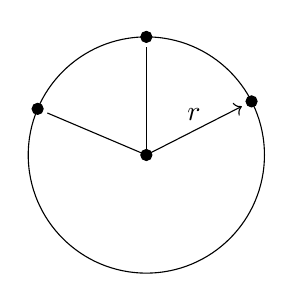
\begin{tikzpicture}
\draw (0,0) circle (1.5cm);
\filldraw[black] (0,0) circle (2pt);
\filldraw[black] (0,0) ++(157:1.5cm) circle[radius=2pt] node(A) {};
\filldraw[black] (0,0) ++(27:1.5cm) circle[radius=2pt] node(B) {};
\filldraw[black] (0,0) ++(90:1.5cm) circle[radius=2pt] node(C) {};


\draw[->] (0,0) -- (B) node[midway,above] {$r$};

\draw (0,0) -- (A);
\draw (0,0) -- (C);
\end{tikzpicture}
Ποια είναι η \(P ( AB \leq r ) \);
\begin{align*}
S&= \left\lbrace 1,2,3,\dots,360  \right\rbrace \\
AB &=\left\lbrace 1,2,3,\dots,120 \right\rbrace \rightarrow\text{ προκύπτει από γεωμετρία}
\end{align*}

\subsection{Αξιώματα \textlatin{Kolmogorov}}
\begin{enumerate}
\item \(0 \leq P(A) \leq 1\)
\item \( P(S) = 1\)
\item \( P(A \cup B) = P(A) + P(B) \)
\begin{tikzpicture}
    \draw[filled] (-0.25,0) circle(1cm) node {$A$}
                  (2.25,0) circle(1cm) node {$B$};
    \draw \boundingbox;
\end{tikzpicture}
\end{enumerate}

\paragraph{}
\(S= \left\lbrace \text{ΚΑ}, \text{SP},\text{MP},\text{KO} \right\rbrace\),
\(A=  \left\lbrace \text{KA}, \text{SP} \right\rbrace\). \(P(A) = \)?

\(P(A) = \frac{2}{4}\) (από κλασικό τρόπο), ή
\(P(\text{KA} \cup \text{SP}) = P(\text{KA})+P(\text{SP}) = \frac{1}{4} + \frac{1}{4}= \frac{1}{2}\), από το 3ο αξίωμα \textlatin{Kolmogorov}.

\subsection{}
\begin{enumerate}
\item \(P(\overline{A}) = 1-P(A)\)

\begin{proof}
\(P(\overline{A} \cup A) = P(S) \implies P(A) + P(\overline{A})=1\)
\end{proof}

\item \(P(\emptyset) = 0\)
\begin{proof}
\begin{align*}
P(\emptyset)&=1-P(\overline{\emptyset}) \\ &= 1-P(S) \\ &= 1-1 =0
\end{align*}
\end{proof}

\item \(P(A) \leq P(B)\)

\begin{tikzpicture}
    \draw[outline] (1,0) circle (1.5cm) node {$A$};
    \draw[outline] (0.5,0.75) circle (0.4cm) node {$B$};
    \draw \boundingbox;
\end{tikzpicture}
\begin{proof}
\begin{align*}
B = (B-A) \cup A \implies \\
P(B) &= P \left( (B-A) \cup A \right) \\
&= P(B-A) + P(A) \geq 0
\end{align*}
\end{proof}

\item \(P(A-B) = P(A) - P(A\cap B)\)

\begin{tikzpicture}
    \begin{scope}
        \clip \firstcircle;
        \draw[filled, even odd rule] \firstcircle node {$A$}
                                     \secondcircle;
    \end{scope}
    \draw[outline] \firstcircle
                   \secondcircle node {$B$};
    \draw \boundingbox;
\end{tikzpicture}

\begin{proof}
\begin{align*}
A = (A-B) \cup (A \cap B) \implies \\
P(A) &= P \left[ (A-B) \cup (A \cap B) \right] \\
&= P(A-B) + P(A \cap B)
\end{align*}
\end{proof}

\item \(P(A \cup B) = P(A) + P(B) - P(A \cap B) \)

% Set A and B
\begin{tikzpicture}
    \begin{scope}
        \clip \firstcircle;
        \fill[filled] \secondcircle;
    \end{scope}
    \draw[outline] \firstcircle node {$A$};
    \draw[outline] \secondcircle node {$B$};
    \draw \boundingbox;
    \node[anchor=south] at (current bounding box.north) {Τομή $A \cap B$};
\end{tikzpicture}


\begin{proof}
\begin{align*}
A \cup B = (A - B) \cup B \implies \\
P(A \cup B) &= P \left[ (A - B) \cup B \right] \\
&= P(A-B) + P(B) \\
&= P(A) -P(A \cap B) + P(B)
\end{align*}
\end{proof}

Μπορεί η παραπάνω σχέση να αποδειχθεί και για περισσότερα από δύο γεγονότα:
\[
P(A \cap B \cap \Gamma ) = P(A)+P(B)+P( \Gamma )-P(A\cap B) - P(A \cap \Gamma ) - P(B\cap\Gamma) + P(A \cap B \cap \Gamma )
\]
\end{enumerate}

\paragraph{}
\begin{circuitikz} \draw
(0,0) node[left] {$A$} to[closing switch=$\Delta_1$] (2,0) to [closing switch=$\Delta_2$] (4,0) node[right] {$B$};
\end{circuitikz}

\(P(\Delta_1)=0.5, \quad P(\Delta_1)=0.3, P(\Delta_1 \cap \Delta_3)=0.1\).\\
Τότε \(P(\Delta) = P(\Delta_1 \cup \Delta_2) = P(\Delta_1) + P(\Delta_2) - P(\Delta_1 \cap \Delta_2) = 0.7\).

\(S =  \left\lbrace \Delta_1\cap\Delta_2,\overline{\Delta_1}\cap\Delta_2,\Delta_1\cap\overline{\Delta_2},\overline{\Delta_1}\cap\overline{\Delta_2} \right\rbrace\)

\subsubsection{}
Για τρία σύνολα \(A,B, \Gamma \): Η πιθανότητα να συμβεί μόνο ένα από αυτά είναι: 
\begin{align*}
& P\left[
\left( A \cap \overline{B} \cap \overline{C} \right) \cap
\left( \overline{A} \cap B \cap \overline{C} \right) \cap
\left( \overline{A} \cap \overline{B} \cap C \right) \right] \\ &= 
P(A \cap \overline{B} \cap \overline{C}) + \dots \\ &= 
P\left[ A - (B \cap \Gamma )\right]
-P(A)-P \left[ A \cap (B \cap \Gamma ) \right] + \dots
\\ &= 
P(A) - P \left[ (A \cap B) \cup (A \cup \Gamma \right]+ \dots  \\ &= 
P(A) - \left( P(A \cap B) + P(A \cap \Gamma) - P(A\cap B\cap \Gamma ) \right)+ \dots  \\\ &=
P(A) - P(A \cap B) - P(A \cap \Gamma) + P(A \cap B \cap \Gamma)+ \dots
\end{align*}

\subsection{Δεσμευμένη πιθανότητα}
\(P(A\cap B) =\)?

\(P(A|B)\): η πιθανότητα να συμβεί το $A$ με την προϋπόθεση ότι $B$, ή η πιθανότητα να συμβεί το $A$, αν γνωρίζουμε ότι συμβαίνει το $B$, σε μια εκτέλεση του πειράματος.

\textit{π.χ.}

\begin{tikzpicture}
    \draw[outline] \firstcircle node {$A$};
    \draw[outline] \secondcircle node {$B$};
    \draw \boundingbox;
    \node at (-0.5,1) {$(3,3)$};
    \node at (-0.65,0.25) {$(3,1)$};
    \node at (-0.5,-1) {$(1,3)$};
    \node at (2,1) {$(2,6)$};
    \node at (3,0.85) {$(6,2)$};
    \node at (3,0.45) {$(2,5)$};
    \node at (3,0.15) {$(5,2)$};
    \node at (3,-0.15) {$(2,4)$};
    \node at (3,-0.45) {$(4,2)$};
    %TODO
\end{tikzpicture}

\(P(A) = \frac{5}{36},\ P(B) = \frac{11}{36}\) \\
Παρατηρώ ότι \(P(A)=\frac{2}{11} = \frac{\frac{N(A\cap B)}{n(s)}}{\frac{N(B)}{N(S)}}\).

Άρα, γενικά:
\[P \left( A | B \right) = \frac{P(A \cap B)}{P(B)} \]

Επομένως:
\begin{align*}
P(A \cap B) &= P(B)P(A|B) \\ &= P(A)P(B|A)
\end{align*}

\begin{itemize}
\item Αν \(A\cap B = \emptyset\), τότε \(P(A|B) = \emptyset\).
\item Αν \(A \subseteq B\), τότε \(P(B|A) = 1\).
\end{itemize}

\subsubsection{Πολλαπλαστιαστικός Κανόνας}
\begin{align*}
P(A_1 \cap A_2 \cap A_3 \cap \cdots \cap A_n) &= \\
&=P(A_1)P(A_2|A_1)P(A_3|A_1\cap A_2)\cdots P(A_n|A_1 \cap \cdots A_n)
\end{align*}

Μπορώ με τη χρήση του πολλαπλασιαστικού κανόνα να εντοπίσω την πιθανότητα 6 ρίψεις ζαριού να έχουν διαφορετικά νούμερα.
\begin{align*}
A_1 &= \left\lbrace \text{στην 1η ρίψη κάποιο νούμερο}  \right\rbrace \\
A_{i \geq 2} &= \left\lbrace \text{στην }i\text{ ρίψη νούμερο διάφορο από } A_{i-1},A_{i-2},\dots,A_1\text{ ρίψη}  \right\rbrace
\\\\
P(A_1 \cap A_2 \cap A_3 \cap A_4 \cap A_5 \cap A_6) &= P(A_1)P(A_2|A_1)P(A_3|A_1\cap A_2)\dots
\end{align*}

\subsection{Θεώρημα Ολικής Πιθανότητας}
%TODO Graph 1
Αν για τα γεγονότα \(A_1,\dots,A_n\) ισχύει:
\begin{itemize}
\item \(A_i \cap A_j = \emptyset\) (ξένα μεταξύ τους)
\item \( \bigcup\limits_{i=1}^k A_i = S \)
\end{itemize}
Ονομάζουμε τα \(A_i\) διαμέριση του \(S\).

Έστω \(B\) ένα σύνολο που τέμνει τη διαμέριση:
\[
B = (B \cap A_1) \cup (B \cap A_2) \cup \cdots \cup (B \cap A_k)
\]
Τότε:
\begin{align*}
P(B)&=P(B \cap A_1)+P(B \cap A_2)+ \cdots + P(B \cap A_k) \\
&=P(A_1)P(B|A_1)+\cdots+P(A_k)P(B|A_k) \\
& = \sum_{i=1}^k P(A_i)P(B|A_i)
\end{align*}

\subsubsection*{Άσκηση}
%TODO Graph2
Επιλέγουμε τυχαία μία κάλπη και μία σφαίρα από την κάλπη. Ποια είναι η πιθανότητα \(P(A)\)να επιλέξω την άσπρη σφαίρα?

Τα \(A_1,A_2,A_3\) αποτελούν διαμέριση. Άρα:
\begin{align*}
P(A) &= \underbrace{P(A_1)}_\frac{1}{3}\underbrace{P(A|A_1)}_0+
\underbrace{P(A_2)}_\frac{1}{3}\underbrace{P(A|A_2)}_\frac{1}{2}
+\underbrace{P(A_3)}_\frac{1}{3}\underbrace{P(A|A_3)}_1 \\
&= 0.50
\end{align*}

\paragraph{Άσκηση}
%TODO Graph 3
\begin{align*}
P(X=1)&=0.60\\P(X=2)&=0.40
\end{align*}
\(P(Y1)=?\)

Τα \(X_1,X_0\) αποτελούν διαμέριση του δειγματικού χώρου.
\begin{align*}
P(Y1)=
\underbrace{P(X1)}_{0.60}
\underbrace{P(Y1|X1)}_{0.90}
+\underbrace{P(X0)}_{0.40}
\underbrace{P(Y1|X0)}_{0.20} = 0.62
\end{align*}

\subsection{Θεώρημα \textlatin{Bayes}}
%TODO Graph 1!
\begin{align*}
P(B)&=P(A_1)P(B|A_1)+\cdots+P(A_k)P(B|A_k) \\
P(A_i|B)&=\frac{P(A_i \cap B)}{P(B)} \\
&=\frac{P(A_i)P(B|A_i)}{P(B)}
\end{align*}
(Πιθανότητα εκ των υστέρων)

\textit{π.χ.}

Από την προηγούμενη άσκηση, ποια είναι η πιθανότητα το αποτέλεσμα να είναι \(1\) αν και η είσοδος είναι \(1\)?
\begin{align*}
P(X1|Y1)=
\frac{P(X1)P(Y1|X1)}{P(Y1)} = 
\frac{0.54}{0.62} > P(X1)=0.6
\end{align*}

Ποια είναι η πιθανότητα \(P(X0|Y1)\)?

\paragraph{}
Στο παράδειγμα με την κάλπη, ποια είναι η \(P(A_3|A)\) (\(P(A_3)=\frac{1}{3}\))
\[
P(A_3|A) = \frac{P(A_3)P(A_1|A_3)}{P(A)} = \frac{\frac{1}{3}\cdot1}{0.50} = \frac{2}{3}
\]
Ομοίως:
\[
P(A_2|A) = \frac{P(A_2)P(A_1|A_2)}{P(A)} = \frac{\frac{1}{3}\cdot\frac{1}{2}}{0.50} = \frac{1}{3}
\]
%TODO Graph 4

\subsection{}
\begin{align*}
P(A) &= 1-P(\overline{A}) \\
P(A \cup B) &= P(A) + P(B) - P (A \cap B) \\
P \left( (A \cup B)| \Gamma \right) &= P(A| \Gamma )+P(B| \Gamma )
- P \left( (A \cap B ) | \Gamma \right)
\end{align*}
Στο παράδειγμα με τα σήματα:
\[
P(X1|Y1) = 1-P(X0|Y1)
\]

\subsection*{}
\begin{circuitikz} \draw
(0,0) node[left] {$A$} -- (1,0) -- (1,1) to[closing switch=$A_1$] (3,1) -- (3,-1) to [closing switch=$A_3$] (2,-1) to [closing switch=$A_2$] (1,-1) -- (1,0);
\draw (3,0) to (4,0) node[right] {$B$};
\end{circuitikz}

\( B = A_1 \cap (A_2 \cup A_3) = \left( A_1 \cap A_2 \right) \cup \left( A_1 \cap A_3 \right) \) (\(Β\) η πιθανότητα διακοπής ρεύματος, \(A_i\) η πιθανότητα να είναι ανοικτός ο \(i\)-οστός διακόπτης.

Άρα:
\begin{align*}
P(B) &= P(A_1 \cap A_2) + P(A_1 \cap A_3) - P(A_1 \cap A_2 \cap A_3) \\
&= P(A_1)P(A_2|A_1)+P(A_1)P(A_3|A_1)-P(A_1)\dots \\
&= P \cdot P + P \cdot P - P^3 \\
&= 2P^2-P^3\quad\text{(αν }P\text{ η πιθανότητα να είναι ανοιχτός ένας διακόπτης)}
\end{align*}

\begin{align*}
P(A_1|B) = \frac{P(A_1 \cap B)}{P(B)}
\end{align*}
Όμως \(A_2 \cap B
= A_1 \cap \left[
\left( A_1 \cap A_2 \right)
\cup
\left( A_1 \cap A_3 \right)
\right]
= (A_1 \cap A_2) \cup (A_1 \cap A_3) = B
\).

Άρα: \(P(A_1|B)= \frac{P(B)}{P(B)} = 1\), κάτι που επιβεβαιώνεται και εμπειρικά.

Ποια είναι η \(P(A_2|B)\)?

\paragraph{Άσκ.}

\begin{tikzpicture}
    \draw[filled] (-1,1) circle(0.5cm) node {$M$}
                  (1,1) circle(0.5cm) node {$M$}
                  (2,-1) circle(0.5cm) node {$A$}
                  (0.5,-1) circle(0.5cm) node {$A$}
                  (-1,-1) circle(0.5cm) node {$A$};
    \draw \boundingbox;
\end{tikzpicture}

\begin{align*}
R &= A_1 \cup (\overline{A_1} \cap \overline{B_2}) \\
P(R) &= P(A_1)+P(\overline{A_1} \cap \overline{B_2})
- \cancelto{\emptyset}{\left[
A_2 \cap (\overline{A_1} \cap \overline{B_2})
\right]} \\
&= \frac{2}{5} \cdot \frac{1}{4}
\end{align*}

Ποια είναι η πιθανότητα να κερδίσει ο \(B\)?

\paragraph{Άσκ.}
%TODO (-2,-2)--(4,2)

\begin{tikzpicture}
    \draw (-1,-1) rectangle (0,1) node {$I$}; %TODO inside
    \draw (0,1) rectangle (3,-1) node {$II$}; %TODO inside
    \draw \boundingbox;
\end{tikzpicture}

Αν \(P(I)=P_1, P(II)=P_2\), ποια είναι η πιθανότητα, αν δεν έχει πληγεί ο 2ος στόχος, να έχει πληγή ο 1ος;

\[
P(I|\overline{II}) =
\frac{P(I \cap \overline{II})}{P(\overline{II})} =
\frac{P(I)\cancelto{1}{P(\overline{II}|I)}}{1-P_2}
\]

\paragraph{Άσκ.}
%TODO Graph 06
\(P(A) = 0.04,\ P(B|A)=0.20\)
\[
\underbrace{R}_\text{πιθανότητα ανύψυσης του βάρους} = \overline{A} \cup (A \cap \overline{B})
\]
\begin{align*}
P(R) &= P(\bar{A})+P(A \cap \overline{B}) -
\cancelto{\emptyset}{P
\left(
\overline{A} \cap (A \cap \overline{B})
\right)
} \\
&= 0.96 + P(A)P(\overline{B}|A) \\
&= 0.96+0.04\cdot0.80
\end{align*}

\paragraph{Άσκηση για το σπίτι}
Σε μια παραγωγή το \(P(A_1)=80\%\) των σιδηροδοκών είναι καλές, και το \(P(A_2)=20\%\) των σιδηροδοκών είναι ελαττωματικές. Το μηχάνημα που πραγματοποιεί τον έλεγχο δεν είναι αξιόπιστο: \(P(\Theta|A_1)=0.10,\ P(\Theta|A_2)=0.80\) (\(\Theta\) η πιθανότητα ο έλεγχος να είναι θετικός).
\begin{enumerate}
\item Ποιο ποσοστό από τις σιδηροδοκούς καταστρέφεται (αν καταστρέφεται κάθε δοκός για την οποία ο έλεγχος είναι θετικός)?
\item Ποιο ποσοστό από αυτές που καταστρέφονται είναι καλές?
\item Ποιο ποσοστό από τις δοκούς που φεύγουν στην αγορά είναι ελαττωματικές?
\item Ποιες θα είναι οι απαντήσεις στα προηγούμενα ερωτήματα αν προτείνουμε δύο ελέγχους \(\Theta_1,\Theta_2\) {\small (καταστρέφεται μόνο αν και οι δύο έλεγχοι είναι θετικοί)}?
\end{enumerate}

\subsection{}

\subsubsection{Ανεξάρτητα \(A,B\)}

\begin{center}
\begin{tikzpicture}
    \draw[outline] \firstcircle node {$A$};
    \draw[outline] \secondcircle node {$B$};
    \draw \boundingbox;
\end{tikzpicture}
\end{center}

\[P(A|B)=P(A) \iff P(A\cap B)=P(A)P(B)\]

\subsubsection{Ασυμβίβαστα \(A,B\)}
\begin{center}
\begin{tikzpicture}
    \draw[filled] (-0.25,0) circle(1cm) node {$A$}
                  (2.25,0) circle(1cm) node {$B$};
    \draw \boundingbox;
\end{tikzpicture}
\end{center}

\[A \cap B = \emptyset,\ P(A|B)=0\]

\textit{π.χ}

Αν \(A,B\) είναι ανεξατητα, ισχύει το ίδιο για τα \(\bar A,B\)?
\begin{proof}
Έχουμε:
\begin{align*}
P(\bar{A}\cap B)
&=
P(B)P(\bar A | B)
\\ &=
P(B) \left( 1 - P(A|B) \right)
\\ &=
P(B) \left( 1-P(A) \right)
\\ &=
P(B)P(\bar A)
\end{align*}
\end{proof}

Μπορείτε να αποδείξετε ότι ισχύει το ίδιο για τα \(\bar A, \bar B\)?

\paragraph{Άσκηση 18}
\[ S =
\begin{cases}
\mathrm A \mathrm B  \Gamma \\ \mathrm A  \Gamma \mathrm B \\\mathrm B \mathrm A  \Gamma \\\mathrm B  \Gamma \mathrm A \\ \Gamma \mathrm A \mathrm B \\ \Gamma \mathrm B \mathrm A 
\end{cases}
\]

\begin{align*}
W &=  \left\lbrace \mathrm A \mathrm B \Gamma , \mathrm A  \Gamma \mathrm B,  \Gamma \mathrm A \mathrm B  \right\rbrace \\
R &=  \left\lbrace \mathrm{A} \mathrm{B} \Gamma , \mathrm A  \Gamma  \mathrm B, \mathrm B A \mathrm  \Gamma  \right\rbrace \\
\text{Πρέπει } \underbrace{P(W \cap R)}_\frac{1}{3} &= 
\underbrace
{
\underbrace{P(W)}_\frac{1}{2}
\underbrace{P(R)}_\frac{1}{2}
}
_\frac{1}{4}
\end{align*}
Άρα τα \(W\) και \(R\) δεν είναι ανεξάρτητα.

\subsection{Τεχνικές Συνδυαστικής}

\subsubsection{Πολλαπλασιαστική αρχή}
Έστω ένα πείραμα στο οποίο ρίχνω ένα νόμισμα και ένα κέρμα.
\begin{align*}
S &= S_1 \underbrace{\times}_\text{καρτεσιανό γινόμενο} S_2 \\
S &=  \left\lbrace \mathrm K  \Gamma  \right\rbrace \times \lbrace 1,2,3,4,5,6 \rbrace \\
&=  \left\lbrace  \left( \mathrm K,1 \right), \left( \mathrm K,2 \right), \dots,  \left( \mathrm K,6  \right), \left(  \Gamma ,1 \right), \left(  \Gamma ,2 \right),\dots, \left(  \Gamma ,6 \right) \right\rbrace
\end{align*}

\paragraph{Άσκηση 8}
\begin{align*}
S &= S_1 \times S_2 \times \cdots \times S_{13} \\
&=
 \left\lbrace 1,2,\times \right\rbrace
 \times
  \left\lbrace 1,2,\times \right\rbrace
  \cdots
   \left\lbrace 1,2,\times \right\rbrace
\end{align*}
\(n=n_1\times n_2 \cdots n_{13}=3^{13}\)

\paragraph{}
Όταν ρίχνω ένα νόμισμα 3 φορές:
\begin{align*}
S &= S_1 \times S_2 \times S_3 \\
&=  \left\lbrace \mathrm K, \Gamma   \right\rbrace \times  \left\lbrace \mathrm K, \Gamma  \right\rbrace\times \left\lbrace \mathrm K, \Gamma  \right\rbrace \\
&=
 \left\lbrace 
 \mathrm K\mathrm K\mathrm K,
 \mathrm K\mathrm K \Gamma ,
 \mathrm K \Gamma \mathrm K,
  \Gamma \mathrm K\mathrm K,
  \mathrm K \Gamma  \Gamma ,
   \Gamma \mathrm K \Gamma ,
    \Gamma  \Gamma \mathrm K,
     \Gamma  \Gamma  \Gamma 
  \right\rbrace
\end{align*}
Παρατηρώ ότι στο καρτεσιανό γινόμενο τα ενδεχόμενα π.χ. \((\mathrm K \mathrm K  \Gamma)\) και \((\Gamma \mathrm K \mathrm  K)\) θεωρούνται διαφορετικά. Αντίστοιχα, σε δύο ρίψεις ενός ζαριού, τα ενδεχόμενα \( (1,2)\), \((2,1)\) είναι διαφορετικά.

\subsubsection{}
Έχω τρία αντικείμενα \(\mathrm A, \mathrm B , \Gamma \). Με πόσους τρόπους μπορώ να τα βάλω στη σειρά?
\[
\begin{cases}
 \mathrm A \mathrm B  \Gamma \\
  \mathrm A \Gamma  \mathrm B \\
     \mathrm B   \mathrm A \Gamma \\
   \mathrm B  \Gamma  \mathrm A\\
    \Gamma  \mathrm A \mathrm B \\
     \Gamma  \mathrm B  \mathrm A
\end{cases}
\]

Για \(n\) αντικείμενα:
\[
n(n-1)(n-2)\cdots 1 = n!
\]

\begin{align*}
\mathrm P(n)&=n!\\
\mathrm P(n,k) &= \frac{n!}{(n-k)!}
\end{align*}

\subsection{Συνδυασμοί}
\[\mathrm C(n,k) = \binom{n}{k}
= \frac{n!}{(n-k)!\ k!}
\]

\textit{π.χ.}
Για τα \( \mathrm A, \mathrm B , \Gamma \) με \(n=3,\ k=2\) (συνδυάζω 3 αντικείμενα ανά 2) έχω:
\[
 \mathrm A \mathrm B  \Gamma 
 \begin{cases}
  \mathrm A \mathrm B \\
   \mathrm A \Gamma \\
    \mathrm B \Gamma 
 \end{cases}
\]

\textit{π.χ.}
Είμαστε 100 φοιτητές, πόσες διαφορετικές επιτροπές των 5 ατόμων μπορώ να φτιάξω?

\paragraph{\textit{Άσκηση}}
Έχουμε 15 καλά και 5 ελαττωματικά ανταλλακτικά. Ποια είναι η πιθανότητα 3 από αυτά να είναι ελαττωματικά?

\subparagraph{Κλασικός τρόπος}
\begin{align*}
P(A)= \frac{N(A)}{N(S)} = \frac{\mathrm C(5,3)}{\mathrm C(20,3)} = \frac{\frac{5!}{(5-3)!\ 3!}}{\frac{20!}{(20-3)!\ 3!}} = \frac{1}{114}
\end{align*}

\subparagraph{Όχι κλασικός τρόπος}
\begin{align*}
A &= \left( A_1 \cap A_2 \cap A_3  \right)
\\
P(A) &=
\underbrace{P(A_1)}_\frac{5}{20}
\underbrace{P(A_2|A_1)}_\frac{4}{19}
\underbrace{P(A_3|A_1 \cap A_2)}_\frac{3}{18} \\
&= \frac{1}{114}
\end{align*}

\subsection{Ασκήσεις}
\paragraph{Ομάδα μπάσκετ από 10 άτομα}
\begin{enumerate}
\item Ομάδα 5 ατόμων: \(\mathrm C(10,5) = \frac{10!}{(10-5)!\;5!}\)
\item Ομάδα 5 ατόμων όπου παίζει ρόλο η σειρά: \(\mathrm P(10,5) = \frac{10!}{(10-5)!}\)
\item
Ομάδα 5 ατόμων που μπορούν να αλλάζουν αριθμό, με 2 \textlatin{standard} παίκτες:
\(\mathrm C(8,3)\cdot 5!\)
\end{enumerate}

\paragraph{Άσκηση 2}
\subparagraph{(α)}
\begin{align*}
S&= \left\lbrace 123,124,125,134,135,145,234,235,245,345 \right\rbrace
\quad \text{(δε με ενδιαφέρει η σειρά)} \\
A&=  \left\lbrace 123 \right\rbrace\\
B&=  \left\lbrace 124,134,234 \right\rbrace \\
 \Gamma &=  \left\lbrace 125,135,145,235,245,345 \right\rbrace
\end{align*}
\subparagraph{(β)} Προφανές

\paragraph{Άσκηση 3}
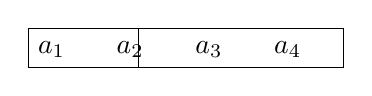
\begin{tikzpicture}
\draw (0,0.5) rectangle (4,0);
\draw (1.4,0) -- (1.4,0.5);
\draw (0,0) node[anchor=south west] {$a_1$};
\draw (1,0) node[anchor=south west] {$a_2$};
\draw (2,0) node[anchor=south west] {$a_3$};
\draw (3,0) node[anchor=south west] {$a_4$};
\end{tikzpicture}
\[
P(A) = \frac{N(A)}{N(S)} = \frac{3}{4}
\]
\begin{align*}
S &= \left\lbrace a_1,a_2,a_3,a_4
 \right\rbrace \\
 A &=  \left\lbrace a_1,a_4 \right\rbrace
 \end{align*}
 \begin{align*}
R &= A_1 \cup (A_2 \cap A_3) \cup A_4 \\
P(R)&=P(A_1)-P(A_2 \cap A_3)+P(A_4)
 \end{align*}

\paragraph{Άσκηση 6}
Για το σπίτι.

\paragraph{Άσκηση 7}
\begin{center}
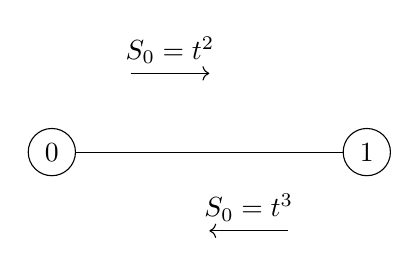
\begin{tikzpicture}
\draw (0,0) circle (3mm) node {$0$};
\draw (4,0) circle (3mm) node {$1$};
\draw (0.3,0) -- (3.7,0);

\draw[->] (1,1)--(2,1) node[midway,above] {$S_0=t^2$};
\draw[->] (3,-1)--(2,-1) node[midway,above] {$S_0=t^3$};
\end{tikzpicture}
\end{center}

\begin{itemize}
\item Από το 0 στο 0.5: \(\Delta t = \sqrt{\frac{1}{2}} \)
\item Από το 0.5 στο 1: \(\Delta t = 1-\sqrt{\frac{1}{2}} \)
\item \(\vdots\)
\end{itemize}

\[ 
P(A)=\frac{(1-\sqrt{\frac{1}{2}})\cdot\left( \frac{1}{3} \right)^\frac{1}{3}}{2}
\]

\paragraph{Άσκηση 9}
Για το σπίτι.

\paragraph{Άσκηση 10}
%TODO Σχήμα

\begin{align*}
P(A_1)&=P(A_2)=P(A_3)=P(A_4)=P \\
P( \Gamma E) &= q \\
R &= (A_1 \cup A_2) \cap \left( (A_3 \cup (  \Gamma E \cap A_4)  \right)
\end{align*}

\paragraph{Άσκηση 11}
%TODO Σχήμα
\begin{gather*}
P(A) = \frac{N(A)}{N(S)} = \frac{12}{100} \\
S =  \left\lbrace 0,1,2,\dots,9 \right\rbrace \\
P(B) = \frac{N(B)}{N(S)} = \frac{6}{40}
\end{gather*}

\paragraph{Άσκηση 12}
\begin{gather*}
K, \Theta\\
P(K) = 0.01 \\
P(\Theta) = 0.02 \\
P(\Theta | K) = 0.08 \\
P \left(  (\Theta - K) \middle| (\Theta \cup K) \right) = ?
\end{gather*}

\begin{align*}
P \left(  (\Theta - K) \middle| (\Theta \cup K) \right) &=
\frac{P \left(  (\Theta - K) \cap (\Theta \cup K) \right)}{P(\Theta \cup K)}
\\
P(\Theta \cup K) &=
P(\Theta)+P(K)-P(\Theta \cap K) \\
&= 0.02+0.01-P(K)P(\Theta | K) \\
&= 0.02+0.01-0.01 \cdot 0.08 \\
&= 0.0292 \\
\text{Άρα }
P \left(  (\Theta - K) \middle| (\Theta \cup K) \right) &=
\frac{P(\Theta - K)}{0.0292} \\
&=
\frac{\overbrace{P(\Theta)}^{0.02} - \overbrace{P(\Theta \cap K)}^{0.0008}}{0.0292}
\\
&\approx 65.75 \%
\end{align*}

\paragraph{Άσκηση 13}
%TODO Σχήμα
\begin{gather*}
P(A) = \frac{N(A)}{N(S)} = \frac{120}{\mathrm C(25,25)}
= \frac{120}{\frac{25!}{(25-2)!}}
\end{gather*}
ή
\begin{align*}
A_1,\ \overline{A_1} \\
P(A_2) &= \underbrace{P(A_2|A_1)}_\frac{4}{24}
\underbrace{P(A_1)}_\frac{5}{25}+
\underbrace{P(A_2|\overline{A_2})}_\frac{5}{25}
\underbrace{P(\overline{A_1})}_\frac{20}{25}
\end{align*}

\paragraph{Άσκηση 15}
\begin{align*}
P(A)=0.10\\
P(B)=0.10\\
P(A\cap B)=0.02
\end{align*}

\begin{align*}
P \left(
(A-B) \cup (B-A)
\right) &= P(A-B)+P(B-A) \\ &=
P(A)-P(A \cap B) + P(B) - P (B \cap A)
\\ &=
0.20 - 2 (0.02) = 0.16
\end{align*}

\begin{align*}
A_0,A_1,A_2
P(E) &=
P(E|A_0)P(A_0)+P(E|A_1)P(A_1)+P(E|A_2)P(A_2)
\\ &=
0.90\cdot 0.82 + 0.70 \cdot 0.16 + 0.40 \cdot 0.02 \\
P(A_0) &= 1 - P(A \cup B)
=
1 -
\big(
\underbrace{
P(A)+P(B)-P(A \cap B)
}_{0.18}
\big) \\
P(A_2|\bar{E}) &=
\frac{\overbrace{P(A_2)}^{0.02} \overbrace{P(\bar{E}|A_2)}^{0.60}}{P(\bar{E})}
\end{align*}

\paragraph{Άσκηση 16}
\begin{gather*}
P(A) = 0.08 \\
P(\overline{A}) = 0.92 \\
P(\Theta | A) = 0.95 \\
P(\Theta | \bar{A}) = 0.05 \\
P(\Theta_1 \cap \Theta_2 | A) = P(\Theta_1|A)P(\Theta_2|A) = 0.95^2 \\
P(\overline{\Theta_1} \cap \overline{\Theta_2}) = P(A)P(\overline{\Theta_1} \cap \overline{\Theta_2} | A)
+ P (\overline{A}) P (\overline{\Theta_1} \cap \overline{\Theta_2}|\overline{A})
= 0.08 \cdot 0.95^2 + 0.92 \left( 0.05^2 \right) \\
P(\overline{A}| \overline{\Theta_1} \cap \overline{\Theta_2})
= P(\overline{A})P\left((\overline{\Theta_1} \cap \overline{\Theta_2})|A\right)
\end{gather*}

\paragraph{Άσκηση 17}
\begin{gather*}
P(A) = 0.60 \\
P(M) = 0.80 \\
P(M|A) = ?
\end{gather*}

\begin{align*}
P(M|A) &= \frac{P(M \cap A)}{P(A)}
\\ &= \frac{;}{0.60}
\\
\underbrace{(M \cup A)}_{\leq 1} &=
\underbrace{P(M)}_{0.80}
+\underbrace{P(M)}_{0.60}
-\underbrace{P(M\cap A)}_{\geq 0.40}
\\ P(M|A) &= \frac{\geq 0.40}{0.60}
\end{align*}

\paragraph{Άσκηση 19}
%TODO Graph
\begin{align*}
P(A) =
\underbrace{P(A|A_1)}_{\frac{1}{4}+\frac{1}{8}=\frac{3}{8}}
\underbrace{P(A_1)}_\frac{1}{4}
+\cdots
+\underbrace{P(A|A_4)}
\underbrace{P(A_4)}
\end{align*}

\paragraph{Άσκηση 20}
%TODO Graph
\begin{align*}
P(A) &= \frac{A}{\pi N \lambda^2} \\
P(\overline{A}) &= 1 -\frac{A}{\pi N \lambda^2} \\
P(\overline{A_1}\cap\overline{A_2}\cap\overline{A_3}\cap\cdots\cap\overline{A_N}) &=
\left(
1- \frac{A}{\pi N \lambda^2}
\right)^N \\
\lim_{N\to \infty} P &= e^{-\frac{A}{\pi \lambda^2}}
\end{align*}

\paragraph{Οι υπόλοιπες ασκήσεις}
για το σπίτι.

\section{Τυχαίες Μεταβλητές}
\[
X,\ Y,\ Z,\ W, \dots
\]

\begin{gather*}
X(s): S \to  \mathbb R _x\\
(5,2) \to 7\\
\mathrm{KK \Gamma } \to 3
\end{gather*}

%TODO Graph 01

\paragraph{}
%TODO Graph 02
\begin{gather*}
X =  \left\lbrace 0,1,2,3 \right\rbrace \\
 \big\lbrace \overbrace{X}^{\mathclap{\text{τυχαία μεταβλητή}}} =
  \underbrace{x}_{\mathclap{\text{τιμές τυχαίας μεταβλητής}}} \big\rbrace
 %\right]
 ,\  \left\lbrace X \subseteq x  \right\rbrace,\
  \left\lbrace  x_1 \subset X \subset x_2  \right\rbrace\\
   \left\lbrace X=1 \right\rbrace \equiv
    \left\lbrace 
    \mathrm{K \Gamma  \Gamma ,\  \Gamma K \Gamma ,\  \Gamma  \Gamma K}
     \right\rbrace\\
      \left\lbrace X \subseteq 2  \right\rbrace \equiv A
\\
P(X=1) = P(\mathrm{K \Gamma  \Gamma ,\  \Gamma K \Gamma ,\  \Gamma  \Gamma K})\\
P\left( X \subseteq 2 \right) = P(A) = \frac{7}{8}\\
P(X=0) = \frac{1}{8}\\
P\left(X \subseteq 1 \right) = \frac{4}{8}
\end{gather*}

\paragraph{Παράδειγμα}
\begin{align*}
S &=  \left\lbrace x \middle| \mathrm{min} \leq x \leq \mathrm{max}  \right\rbrace \\
X &=  \left\lbrace x \middle| \mathrm{min} \leq x \leq \mathrm{max}  \right\rbrace \\
Y &=  \left\lbrace y \middle| \dots  \right\rbrace \\
\end{align*}

\subsubsection{Συνάρτηση μάζας πιθανότητας (\textlatin{Probability Mass Function} - σμπ)}
\(
X =  \left\lbrace x_1,x_2,\dots,x_n \right\rbrace
\)
\[
f(x_i) = P(X=x_i) = P_i
\]

\paragraph{Παράδειγμα}
\begin{align*}
S &=  \left\lbrace \mathrm{\epsilon,\ \kappa \epsilon,\ \kappa \kappa \epsilon,\kappa \kappa \kappa \epsilon},\dots  \right\rbrace \\
X &=  \left\lbrace 1, 2, 3,\ \dots  \right\rbrace\\
P(\epsilon) &= 0.01
\end{align*}

\[
\begin{array}{r|l}
P(X=x_i) & x_i\\
\hline
P(X=1)=P(\epsilon)=0.01 & 1 \\
P(X=2)=P(k\epsilon)=\quad & 2 \\
\end{array}
\implies
\begin{array}{r|l}
P(X=x_i) & x_i\\
\hline
0.01 & 1\\
0.01(0.99) & 2 \\
0.01(0.99)^2 & 3 \\
0.01(0.99)^3 & 4 \\
\vdots & \vdots \\
0.01(0.99)^\lambda & \lambda
\end{array}
\]

\paragraph{Ιδιότητες}
\begin{enumerate}
\item \(f(x_i) \geq 0\)
\item \(\sum\limits_{x_i=0}^\infty f(x_i) = 1\) (ισχύει στο παράδειγμα?)
\end{enumerate}

\subsubsection{Συνάρτηση Πυκνότητας Πιθανότητας}
%TODO Zioutas Graph 04
\begin{enumerate}
\item \(f(x) \geq 0\)
\item \(P(x_1 < X < x_2) = \int\limits_{x_1}^{x_2} f(x) \dif x\)
\item \(\int\limits_{-\infty}^{+\infty} \dif x = 1\)
\end{enumerate}

\[
P(X=x) \cong P (x-\delta\epsilon \leq X \leq x+\delta\epsilon) = \int_{x-\delta\epsilon}^{x+\delta\epsilon} f(x) \dif x
\]

Να σημειωθεί ότι \(P(X=x) = 0\), αλλά το \((X=x)\) δεν είναι αδύνατο, αφού \((X=x) \equiv  \left\lbrace x \right\rbrace\).

%TODO Zioutas Graph 05
\[
\int_a^b f(x) \dif x = 1
\]

\[
\int_a^b c \dif x =c [x]_a^b = 1 \implies c = \frac{1}{b-a}
\]

\paragraph{Παράδειγμα}
\[
P(X \geq x_1) = \int_{x_1}^\infty \frac{1}{2}e^{-\frac{x}{2}} \dif x = e^{-\frac{x_1}{2}}
\]

\[
\int_0^\infty f(x)\dif x = 1
\]
\[
\int_0^\infty Ae^{-\frac{x}{2}} \dif x = -A2\left[ e^{-\frac{x}{2}}\right]_0^\infty = 2A =1
\implies A=\frac{1}{2}
\]

\subsection{Αθροιστική Πιθανότητα - Συνάρτηση Κατανομής}
\[
F(x) = P(X \leq x) = \int_{\infty}^x f(u) \dif u = \sum_{x_i \leq X} =P(X=x_i)
\]

\[
f(x)=
\begin{cases}
\frac{1}{8} \quad& x=0\\
\frac{3}{8} \quad& x=1\\
\frac{3}{8} \quad& x=2\\
\frac{1}{8} \quad& x=3
\end{cases}
\qquad
F(x)=
\begin{cases}
0 \quad& x=0\\
\frac{1}{8} \quad& x<0\\
\frac{4}{8} \quad& 1 \leq x < 2\\
\frac{7}{8} \quad& 2 \leq x < 3\\
\frac{8}{8} \quad& 3\leq x
\end{cases}
\]
\[
F(x) = P(X \leq x)
\]

%TODO Zioutas Graph 08
\begin{align*}
F(1) &= P(x \leq 1) =\frac{4}{8}\\
F(0.5) &= P(x=0) = \frac{1}{8}
\end{align*}

\paragraph{Σε συνεχή μεταβλητή...}
%TODO Zioutas Graph 09
\[
F(x) = P(X \leq x) = \int_a^x \frac{1}{1-ba} \dif x = \frac{x-a}{b-a}
\]

\[
F(x) = \begin{cases}
0 &\quad x<a\\
\frac{x-a}{b-a} &\quad a\leq x\leq b \\
1 &\quad x>b
\end{cases}
\]

\subsubsection{Ιδιότητες}
\begin{enumerate}
\item \(F(-\infty)=0,\ F(+\infty)=1\)
\item \( x_1<x_2 \implies F(x_1)<F(x_2)\)
\item \(F(x^+)=F(x)\)
\item \(\begin{cases}
f(x)=\od{F(x)}{x}\quad F(x)=\int_{-\infty}^x f(u)\dif u \\
f(x_i) = F(x_i)-F(x_{i-1}) \\
F(x) = \sum\limits_{x_i \leq x} f(x_i)\\
P(x_1 < X \leq x_2) = F(x_2)-F(x_1)
\end{cases}\)
\end{enumerate}

\subsubsection{Μικτού τύπου}
%TODO Zioutas Graph 03

\begin{gather*}
P(X=x_1)=P_1\\
P(X=x_2)=P_2
\end{gather*}

\paragraph{Παράδειγμα}
%TODO Zioutas Graph 04

Αν γνωρίζουμε επιπλέον ότι \(P(X\leq1)=\frac{2}{5}\), τότε προκύπτει \(\int_0^1 \lambda_1e^{-\lambda_2x}\dif x = \frac{2}{5}\), και μπορούμε στο σπίτι να βρούμε τα \(\lambda_1,\lambda_2\).

\subsection{Ασκήσεις (Τυχαίες Μεταβλητές ΑΣΚΗΣΕΙΣ-ΠΡΟΒΛΗΜΑΤΑ)}
\subsubsection*{1}
\begin{align*}
P(X>1) &= 1-P(X\leq1) \\
&= 1-F(1)\\
&= 1-\left(1-\exp(-1^2)\right)\\
&= \cancel{1}-\cancel{1}+e^{-1}
\end{align*}

\subsubsection*{2}
\paragraph{(α)}
\begin{align*}
\int_0^2 f(x)\dif x &= 1 \\
&\implies c\left(4 \left[\frac{x^2}{2}\right]_0^2 - 2 \left[\frac{x^3}{3}\right]_0^2\right)=1\\
&\implies c=...
\end{align*}

\paragraph{(β)}
\begin{align*}
P(x>1) &= 1-P(X\leq1) \\
&=1-\int_0^1f(x)\dif x
\end{align*}

\subsubsection*{3}
Για το σπίτι

\subsubsection*{4}
\paragraph{(α)}

\[
F(x) = \begin{cases}
0&\qquad x<0\\
\frac{x}{k}&0\leq x\leq 5\\
1&x>5
\end{cases}
\]

%TODO Zioutas Graph 05

\[
f(x) = \begin{cases}
0&\qquad x<0\\
\od{F(x)}{x}=\frac{1}{k}&\qquad 0\leq x\leq 5\\
0&\qquad x>5
\end{cases}
\]

%TODO Zioutas Graph 06
\[
\int_0^5 \frac{1}{k}\dif x=\frac{1}{k}\left[ x\right]_0^5=\frac{5}{k}=1
\implies k=5
\]

\paragraph{(β)}
\[
F(x)=\begin{cases}
0\qquad& x<-1\\
\sfrac{x^3}{4}+0.5\quad&-1\leq x < 1\\
1& x\geq 1
\end{cases}
\]

%TODO Zioutas Graph 07
\[
f(x)=\begin{cases}
P(X=-1)=\frac{1}{4} \qquad& x=-1\\
\od{F(x)}{x}=\frac{3x^2}{4}& x<1\\
P(X=1)=\frac{1}{4}
\end{cases}
\]

\begin{gather*}
\int_0^1 f(x)\dif x = 1;\\
F() = \int_0^x f(u)\dif u
\end{gather*}


\subsubsection*{5}
Για το σπίτι

\subsubsection*{6}
\begin{gather*}
\mathrm P(A)=0.5\\
\mathrm P(B)=0.8\\
\mathrm P(\Gamma)=0.2\\
X= \left\lbrace 0,1,2,3 \right\rbrace
\end{gather*}

%TODO Zioutas Graph 08
\begin{align*}
P(X=0)&=1-P(A\cup B\cup  \Gamma )\\
P(X=1)&=P(A\cap\bar B\cap\bar \Gamma )+P(\bar A \cap B \cap\bar\Gamma)+P(\bar A\cap\bar B\cap \Gamma )\\
&= P(A)P(\bar B)P(\bar \Gamma)+\dots\\
P(X=2)&=\dots\\
P(X=3)&=\dots
\end{align*}

\subsubsection*{8}
%TODO Zioutas Graph 09
\begin{gather*}
X= \left\lbrace -2,0,2 \right\rbrace
\end{gather*}

Οι πιθανότητες είναι ίσες με τα αντίστοιχα άλματα της αθροιστικής:
\begin{align*}
P(X=-2)&=0.2\\
P(X=0)&=0.5\\
P(X=2)&=0.3
\end{align*}


\subsubsection*{9}
%TODO Zioutas Graph 10
\paragraph{(α)}
\[
P(X\geq3000) = \int_{3000}^\infty f(x)\dif x =\boxed{e^{-\frac{1}{1000}\cdot3000}}
\]
\paragraph{(β)}
\[
P(X<1000)=\int_0^{1000}f(x)\dif x = 1-e^{-\frac{1000}{1000}}
\]
\paragraph{(γ)}
\[
\int_{1000}^{2000}
\]
\paragraph{(δ)}
\begin{align*}
P(X\leq x) &= 0.10\\
&= 1-e^{-\frac{1}{1000}x}=0.10\\
\implies& x=\dots
\end{align*}

\subsubsection*{10}

\[
f(x) = \begin{cases}
c\qquad& [-a.-\sfrac{a}{2}]\\
c&[\sfrac{a}{2},a]\\
0&\text{αλλού}
\end{cases}
\]

%TODO Zioutas Graph 11
\(P(X\leq3=0.75)\)

...

\[
f(x)= \begin{cases}
\int_{-a}^x c\dif x \qquad& -a<x<-\sfrac{a}{2}\\
\int_{-a}^{-\sfrac{a}{2}} c\dif x & -\sfrac{a}{2}<x<\sfrac{a}{2}\\
 \int_{-a}^{-\sfrac{a}{2}} c\dif x + \int_{\sfrac{a}{2}}^x c \dif x  & \sfrac{a}{2}<x<a \\
1 & x>a
\end{cases}
\]

\subsection{Χαρακτηριστικά}
\begin{enumerate}
\item Μέση Τιμή \(\mu_x,\ E(x)\)
\item Διακύμανση \(\sigma_x^2,\ \mathrm{Var}(X)\)
\item \(x_p,\ M,\ T\)
\end{enumerate}

\subsubsection{Μέση Τιμή (\textlatin{Mean})}

\begin{align*}
\mu_x=E(X)&=\int_{-\infty}^\infty x f(x)\dif x\\
&=\sum_{x_i}x_i f(x_i)
\end{align*}

\paragraph{π.χ.}
\begin{align*}
X&= \left\lbrace 1,2,3,4,5,6 \right\rbrace\\
f(x_i)&=\frac{1}{6}\\
E(X)&=\frac{1}{6}(1+2+\dots+6)=3.5
\end{align*}
%TODO Zioutas Graph 01
\[
E(X)=\int_0^\infty x\lambda e^{-\lambda x}\dif x = \frac{1}{\lambda}
\]

\paragraph{Ιδιότητες}
\begin{itemize}
\item \begin{align*}
E(aX+\beta) &=\int_{-\infty}^\infty (ax+\beta)f(x)\dif x\\
&= aE(x)+\beta
\end{align*}
\item \(
E\left(g(x)\right) = \int_{-\infty}^\infty g(x)f(x)\dif x
\)
\end{itemize}
%TODO Zioutas Graph 02
\begin{align*}
f(x)&=\begin{cases}
c=\frac{1}{\beta-a}\quad& a<x<\beta\\
0&\text{αλλού}
\end{cases}\\
E(X)&=\int_a^\beta x\frac{1}{b-a}\dif x\\
&= \frac{a+\beta}{2}
\end{align*}
%TODO Zioutas Graph 03
\begin{align*}
E(X)=\int_0^1 x(1)\dif x = 0.5\\
E(X^2)=\int_0^1 x^2(1)\dif x = \frac{1}{3}
\end{align*}
\begin{align*}
X: [-1,1] \cap \mathbb Z \qquad& E(X)=-1\left(\frac{1}{2}\right)+1\left(\frac{1}{2}\right)\\
Y: [-1000,1000] \cap \mathbb Z \qquad& E(Y)=0
\end{align*}
Πρέπει να ορίσουμε ένα μέγεθος με το οποίο να μπορούμε να συγκρίνουμε την ομοιογένεια/διακύμανση των τιμών.

\begin{align*}
E(X-\mu_x)&=0\\
E\left(|X-\mu_x|\right) &= \dots
\end{align*}

\subsubsection{Διακύμανση \(\sigma^2_x, \ \mathrm{Var}(X)\)}
\begin{align*}
\sigma_x^2 &= E \left[ (X-\mu_x)^2\right] \\
&= \int_{-\infty}^\infty (x-\mu)^2f(x)\dif x
\end{align*}

\begin{align*}
\mathrm{Var}(x) &= E \left[(x-\mu)\right]^2
\\ &= E(X^2)-\mu_x^2
\\ &= \int x^2f(x)\dif x - \mu_x^2
\end{align*}

\begin{align*}
\mathrm{Var}(aX+\beta) &= E\left[
\left(
aX+\beta -(a\mu_x+\beta)
\right)^2
\right] \\
&= \dots = a^2\mathrm{Var}(X)
\end{align*}

%TODO Zioutas Graph 01
\begin{align*}
E(X) &= \frac{1}{\lambda} \\
\mathrm{Var}(X) &= E(X^2)-\left(\frac{1}{\lambda}\right)^2 \\
&= \int_0^\infty x^2\lambda e^{-\lambda x} \dif x - \left(
\frac{1}{\lambda}^2
\right) = \dots = \left( \frac{1}{\lambda} \right)^2
\end{align*}

%TODO Zioutas Graph 02
\begin{align*}
E(X)&=\frac{a+\beta}{2}\\
\mathrm{Var}(X)&=E(X^2)-\left(\frac{a+\beta}{2}\right)^2=\text{ για το σπίτι}
\end{align*}

\subsubsection{Τυπική απόκλιση}
\begin{align*}
X&=\dots\\
f(x)&=\dots\\
\mathrm E(X) &= \mu_x\\
\mathrm{Var}(X) &= \sigma_x^2\\
\text{Τυπική απόκλιση } \sigma_x &= \sqrt{\sigma_x^2}
\end{align*}

\paragraph{Τυποποίηση}
\[
X^* = \frac{X-\mu_x}{\sigma_x}
\]

Τότε:
\begin{align*}
E(X^*)=0 \quad &\text{(να αποδειχθεί)}\\
\mathrm{Var}(X^*)=1 \quad &\text{(να αποδειχθεί)}
\end{align*}

\subsubsection{\(x_p=P\) ποσοστιαίο σημείο}
%TODO Zioutas Graph 04

\subsubsection{Διάμεσος (\textlatin{Median})}
\begin{gather*}
x_{0.5} = M\\
P(X \leq M) = P(X\geq M) = 0.5
\end{gather*}

\subsubsection{Επικρατέστερη Τιμή}
%TODO Zioutas Graph 05

\paragraph{π.χ.}
\begin{align*}
f(x)=\begin{cases}
\frac{4x(9-x^2)}{81}\quad& 0 \leq x \leq 3\\
0 & \text{αλλού}
\end{cases}
\end{align*}

\(T=; \quad \od{f(x)}{x}=0\)

\(M=; \quad F(M)=0.5 \implies M=\dots\)

\(\mu_x = ;\)

\paragraph{π.χ}
\begin{gather*}
X =  \left\lbrace 1,2,3,\dots \right\rbrace \\
f(x_i) = P(X=x_i) = \frac{1}{2x_i}\\
T = 1\\
M = \text{οποιαδήποτε τιμή μεταξύ του 1 και 2}\\
\mu_x = \sum_{x_i=1}^\infty x_i \frac{1}{2x_i} = \dots = 2 
\end{gather*}

\paragraph{Άσκηση}
%TODO Zioutas Graph 06
%TODO Zioutas Graph 07

\[
f(x)=\begin{cases}
0&x<-2\\ax+\beta&-2\leq x\leq0\\c&0\leq x\leq4\\0&x<4
\end{cases}
\qquad
\xRightarrow{\dots} 
f(x)=\begin{cases}
0&x<-2\\0.1x+0.2&-2\leq x\leq0\\c&0\leq x\leq4\\0&x<4
\end{cases}
\]

\[
F(x)=\begin{cases}
0&x<-2\\
\int_{-2}^x\ = 0.05x^2+0.2x+0.2&-2\leq x < 0\\
\attnboxed{\frac{1}{5}}+\displaystyle\int_0^x\textstyle \frac{1}{5}\dif u = 0.2+0.2x & 0 \leq x < 4\\
1&x\geq 4
\end{cases}
\]

\begin{attnbox}{}
\begin{align*}
P(X\leq M) &= 0.50\\
F(M) &= 0.2+0.2Μ = 0.5 \implies \boxed{M=1.5} \quad \text{(με το μάτι επιλέγω κλάδο)}
\end{align*}

Ποια είναι η μέση τιμή της \(Y=g(x)=\sfrac{10}{6}(x)+\sfrac{20}{6}\)?

\begin{align*}
Y&=g(x)\\
E(y)&=E\left(g(x)\right)=\int_{-2}^0 g(x)f_1(x)\dif x + \int_0^4 g(x)f_2(x)\dif x
\\
&= \dots = \boxed{\frac{88}{18}}
\end{align*}
\end{attnbox}

\paragraph{Άσκηση 11}
%TODO Zioutas Graph 08
\[
f(x)=\begin{cases}
P(X=0)=\frac{2}{3}\quad&x=0\\
c=\frac{2}{3}& 0 < x \leq 0.5
\end{cases}
\]
\begin{gather*}
E(X)=\cancelto{0}{0\cdot\frac{2}{3}}+\int_0^{0.5}x\left(\frac{2}{3}\right)\dif x = \frac{2}{3}\left[
\frac{x^2}{2}
\right]_0^{10.5}=\dots
\end{gather*}

\paragraph{Άσκηση 13}
Για το σπίτι

\subsection{Χρήσιμες Κατανομές}
\begin{gather*}
X,\ f(x),\ F(x),\ E(x)\\
P(X \leq x) = \int_{-\infty}^x f(u) \dif u
\end{gather*}
%TODO Zioutas Graph 01
\begin{enumerate}
\item \textlatin{Bernoulli}
\item Διωνυμική
\item Γεωμετρική
\item \textlatin{Pascal}
\item \textlatin{Poisson}
\end{enumerate}

\subsubsection{\textlatin{Bernoulli}}
\begin{align*}
S &=  \left\lbrace \overbrace{A}^{\text{"επιτυχές γεγονός"}}, \bar{A}  \right\rbrace\\
X &=  \left\lbrace 1, 0 \right\rbrace\\
P(A) &= p\\
P(\bar{A}) &= 1-p\\
f(x_i): P(X=1)&=p\\
P(X=0)&=1-p\\
E(X)&=1 \cdot p + 0\, (1-p) = p\\
\mathrm{Var}[X] &= \mathrm E(X^2)-p^2 = p \cdot (1-p)
\end{align*}


\subsubsection{Διωνυμική}
\begin{align*}
X =&  \left\lbrace 
\begin{matrix}
\text{αριθμός εμφάνισης $A$}\\
\text{σε $n$ δοκιμές}
\end{matrix}
 \right\rbrace\\
 X=&  \left\lbrace 0,1,2,\dots,n \right\rbrace\\
 P\big(X=x\big)=&\binom{n}{x}\; p^x(1-p)^{n-x}\\
 \sum_{x=0}^n \binom{n}{x}p^x(1-p)^{n-x} =& \left(p+(1-p)\right)^n=1
\end{align*}
\begin{align*}
\mathrm E(X)=&\sum_{x=0}^n x \binom{n}{x}p^x(1-p)^{n-x}
\\ =& \cdots \\ =&\; np
\end{align*}

\paragraph{Παράδειγμα}
Ρίχνουμε ένα ζάρι $n=20$ φορές. Ποια είναι η πιθανότητα να έχουμε 5 άσσους?
\begin{align*}
P(A) &= \frac{1}{6}\\
X &=  \left\lbrace 0,1,2,\dots,20 \right\rbrace\\
P(X=S) =& \binom{20}{5} \left( \frac{1}{6}\right)^5 \left(\frac{5}{6}\right)^{15}
\end{align*}

\paragraph{}
\begin{gather*}
n=100 \text{ στήλες}\\
p = 0.01 \text{ ελαττωματική}\\
P(X \leq 4) = \sum_{x=0}^4 \binom{100}{x} 0.01^x (1-0.01)^{100-x} \\
X=  \left\lbrace 0,1,2,\dots,100 \right\rbrace
\end{gather*}

\subsubsection{Γεωμετρική}
\begin{align*}
X &=  \left\lbrace 
\begin{matrix}
\text{αριθμός δοκιμών}\\
\text{μέχρι εμφάνισης του $A$}\\
\text{για πρώτη φορά}
\end{matrix}
 \right\rbrace\\
X &=  \left\lbrace 1,2,3,4,\dots \right\rbrace\\
P(X=x) &= P(\underbrace{\bar{A}\bar{A}\bar{A}\cdots \bar{A}\bar{A}}_{\mathclap{x-1 \text{ φορές } \bar{A}}} A)
\\ &= (1-p)^{x-1}p \\
\sum_{x=1}^\infty (1-p)^{x-1}p=1\\
\text{Περίοδος επαναφοράς} \mathrm E(X) &=
\frac{1}{p}
\end{align*}

\paragraph{Παράδειγμα}
\begin{align*}
E(X)&=2.5=\frac{1}{p}\implies p - 0.4\\
P(X=1)&=(1-p)^{x-1}p\\&=\frac{1}{3}p\\
P(X<3)=1-P(X\leq3),\quad P(X\leq3)&=\sum_{x=1}^3 (1-p)^{x-1}p
\end{align*}

\subsubsection{\textlatin{Pascal}}
\begin{align*}
X_r&=  \left\lbrace 
\begin{matrix}
\text{αριθμός δοκιμών}\\
\text{μέχρι $r$ εμφανίσεις του $A$}
\end{matrix}
 \right\rbrace\\
X_r&= \left\lbrace r,\ r+1,\ \dots \right\rbrace\\
P(X_r=x) =& \binom{x-1}{r-1}(1-p)^{(x-1)-(r-1)}p^r
\end{align*}

\paragraph{Παράδειγμα}
\begin{gather*}
p = 0.00005 \text{ πιθανότητα να χαλάσει ο υπολογιστής}\\
\text{6 ωρών}\\
X_3= \left\lbrace 
3,4,5,6,7,8,\dots
 \right\rbrace\\
 P(X_3>6) = 1-P(X_3 \leq 6)
 \\
 ω = toast
\end{gather*}

\paragraph{}
%TODO Zioutas Graph 02
\begin{gather*}
\Big(X_{51}=101\Big)=\cdots
\end{gather*}


\subsubsection{\textlatin{Poisson}}
\begin{align*}
X_t= \left\lbrace 
\begin{matrix}
\text{αριθμός εμφάνισης $A$}\\
\text{σε διάστημα $t$}
\end{matrix}
 \right\rbrace
\end{align*}
\begin{enumerate}
\item \(\Delta t\)
\item \(P(X_{\Delta t}=1)=\Delta t \cdot \lambda\)
\item \(t_1,\ t_2\)
\end{enumerate}

\begin{gather*}
P(X_t=t) = e^{-\lambda t} \frac{(\lambda t)^x}{x!}\\
E(X_t) = \sum_{x=0}^\infty x e^{-\lambda t} \frac{(\lambda t)^x}{x!} = \dots = \lambda t\\
E(X_1)=\lambda\\
\sigma^2_{x_t} =\lambda t
\end{gather*}

\paragraph{Παράδειγμα}
\begin{gather*}
\lambda = \frac{16}{80} \text{ σεισμοί/χρόνο}\\
X_{t=10}= \left\lbrace 0,1,2,\dots \right\rbrace\\
P(X_{t=10} \geq 1) = 1- P(X_{t=10}=0)\\
P(X_{t=10} = 4) = e^{-\lambda t} \frac{(\lambda t)^4}{4!}=1-e^{-\frac{16}{80}(10)}\frac{2^0}{0!}=1-e^{-2}\\
E(X_{t=20})=\frac{16}{80}20=4
\end{gather*}


\paragraph{Απόδειξη}
\begin{align*}
\Delta t \text{ μικρό}\\
P(A) = P = \lambda \Delta t \to 0\\
n=\frac{t}{\Delta t} \to \infty
\end{align*}

\begin{align*}
P(X_t=x) &= \binom{n}{x} p^x (1-p)^{n-x}\\
&= \frac{n!}{(n-x)!\; x} \left( \frac{t}{n} \right)^x \left(1-\frac{\lambda t}{n}\right)^n (1-p)^{-x}\\
&= \frac{1}{x!} \left( \frac{t\lambda}{n}\right)^x e^{-\lambda t}\\
E(X_t)&=n\lambda \Delta t
\\ &= n\lambda \frac{t}{n}
\end{align*}

\paragraph{Άσκηση 3}
\[
\begin{array}{cc}
n=5
\qquad&\qquad
n=20
\\p=0.80&p=0.20\\X= \left\lbrace 0,1,2,3,4,5 \right\rbrace
& X= \left\lbrace 0,1,2,\dots,20 \right\rbrace\\
P(X=4) = \binom{5}{4} p^4(1-p)^{5-4} = 40.96\%
\qquad& P(X>4) = 1-P(X\leq4) = 1-\sum_{x=0}^4 \binom{20}{x} p^x(1-p)^{20-x}
\end{array}
\]

\paragraph{Άσκηση 4}
%TODO Zioutas Graph 03
\begin{align*}
p&=\frac{12}{60}=0.20\\
X&= \left\lbrace 0,1,2,\dots,10 \right\rbrace\\
n&=10\\
P(X\leq \kappa) &= 0.90\\
\sum_{x=0}^\kappa \binom{10}{x} p^x(1-p)^{10-x} &=0.90
\end{align*}

Προκύπτει με μέθοδο δοκιμής και λάθους ότι για $\kappa=4$ η πιθανότητα ξεπερνάει το 0.90.

\paragraph{Άσκηση 8}
\begin{align*}
\lambda &= ^{100}/_\text{λεπτό}\\
X_t &=  \left\lbrace 0,1,2,\dots \right\rbrace\\
P(X_{t=1}=100) &= e^{-100} \frac{100^{100}}{100!}\\
P\left(X_{t=\frac{1}{60}}=10\right) &= e^{-100\left(\frac{1}{60}\right)} \frac{\left(100\frac{1}{60}\right)}{10!}
\end{align*}

\paragraph{Άσκηση 7}
\begin{align*}
n & \qquad \text{Διωνυμική} X= \left\lbrace 0,1,2,\dots,n \right\rbrace\\
P(\kappa = 0) &= \frac{5}{12}\\
P(\kappa = 1) &= \frac{1}{3}\\
P(\kappa = 2) &= \frac{1}{4}\\
 \hline & 1\\
 P(X=0) &= \binom{n}{0}p^0(1-p)^{n-0}\\
 P(X=1) &= \binom{n}{1}p^1(1-p)^{n-1}\\
 P(X=2) &= \binom{n}{2}p^2(1-p)^{n-2}\\
 P(E) &= 
 P\left(E\middle| \left\lbrace \kappa=0  \right\rbrace\right)P(\kappa=0)
 +P\left(E\middle| \left\lbrace \kappa=1  \right\rbrace\right)P(\kappa=1)
 +P\left(E\middle| \left\lbrace \kappa=2  \right\rbrace\right)P(\kappa=2)
 \\ &=
 P(X=0)\frac{5}{12}+P(X=1)\frac{1}{3}+P(X=2)\frac{1}{4}
 \\ &= \dots
\end{align*}

\paragraph{Άσκηση 9}
\begin{align*}
P(X_t=0) &= e^{-\lambda t} \frac{(\lambda t)^0}{0!} = 0.90 \implies \dots
\end{align*}

\paragraph{Άσκηση 15}
\begin{align*}
p &= 0.05\\
n &= 52\\
\text{Αριθμός αυτών που θα ακυρώσουν } X &=  \left\lbrace 0,1,2,\dots,52 \right\rbrace\\
P(X\geq2) &= 1 - P(X\leq1) = 1-\binom{52}{0}p^0(1-p)^{52-0}-\binom{52}{1}p^1(1-p)^{52-1}\\
\boxed{1-p^*} \quad Y= \left\lbrace 1,2,\dots \right\rbrace \\ \mathrm{E}(y)=\frac{1}{1-p^*}=\boxed{10} \implies \boxed{p*} = p(X \geq k) = \dots
\end{align*}

\subsection{Συνεχής \(X\)}
\begin{enumerate}
	\item Ομοιόμορφη
	\item Εκθετική
	\item Κανονική
\end{enumerate}

\subsubsection{Ομοιόμορφη}
%TODO Zioutas Graph 01
\begin{align*}
c &= \frac{1}{\beta-a} \\
F(x) &= P(X \leq x) \\
&= \frac{x-a}{\beta-a} \\
\mathrm E(x) &= \frac{a+\beta}{2} \\
\sigma^2_x = \frac{(\beta-a)^2}{12}
\end{align*}

\[
X \sim U[0,1]
\]

\paragraph{title}
%TODO Zioutas Graph 02

\begin{align*}
F_y(y) &= 1-e^{-y\lambda }\\
x_1 &= 1-e^{-y_2\lambda } \\
e^{-y_1\lambda }&=-x_1+1\\
y_1\lambda &= \ln (1-x_1) \implies y_1 = \frac{1}{\lambda} \ln (1-x_1)
\end{align*}



\subsubsection{Εκθετική}
%TODO Zioutas Graph 03
\[
T = \left\lbrace
\text{χρόνος ανάμεσα σε διαδοχικά \(A\)}
\right\rbrace
\]
\begin{gather*}
X_t = \left\lbrace 0,1,2,\dots \right\rbrace\\
P(X_t=x) = e^{-\lambda t} \frac{(\lambda t)^x}{x!} \\
E(X_t)=\lambda t\\
f_T(t) = \od{F_T(t)}{t}
\end{gather*}
\begin{align*}
F_T(t) &= P(T \leq t) =
\\ &=
1-P(T>t)
\\ &=
1-e^{-\lambda t}\cancelto{0}{\frac{(\lambda t)^0}{0!}}
\end{align*}
\begin{align*}
F_T(t) &= 1-e^{-\lambda t} \implies \\
\implies f_T(t) &= \lambda e^{-\lambda}t\\
\mathrm E(T) &= \frac{1}{\lambda }\\
\mathrm{Var}(T) &= \frac{1}{\lambda ^2}
\end{align*}

\paragraph{Παράδειγμα}
\begin{align*}
\lambda &= \frac{16}{125} = 0.128 \text{ σεισμοί/χρόνο} \\
P(X \leq 2) &= 1-e^{-\lambda (2)} \\
&= 1-e^{-0.128 (2)} \\
&\approx 22.6\%
\end{align*}
\begin{gather*}
Y_{t=2} = \left\lbrace 0,1,2,\dots \right\rbrace\\
\text{\textlatin{Poisson}} \\
P(Y_{t=2} \geq 1) = 1 - P(Y_{t=2} = -) = 1 - e^{-\lambda (t)} \cancelto{0}{\frac{\lambda (t)}{0!}}
\end{gather*}

Περίοδος επαναφοράς σεισμού: \(\frac{1}{\lambda } \approx 8 \text{ χρόνια}\)

\paragraph{Έλλειψη μνήμης}
\begin{align*}
P(X > t_1 + t_2 | X > t_1) &= \frac{P(X>t_1+t_2)}{P(X>t_1)}
\\ &= \frac{e^{-(t_1+t_2)\lambda }}{e^{-t_1 \lambda }} \\
&= e^{-t_2\lambda } = P(X> t_2)
\end{align*}

\subsubsection{Κανονική \textlatin{Gauss}}
\[
X \sim N(\mu, \sigma^2)
\]

\begin{align*}
f(x) &= \frac{1}{\sqrt{2\pi}\sigma} e^{-\frac{1}{2} \left(\frac{x-\mu}{\sigma} \right)^2 }\\
\mathrm E(X) &= \int_{-\infty}^\infty f(x) x \dif x = \dots = \mu\\
\mathrm{Var}(X) &= \sigma_x^2 = \dots = \sigma^2 \\
\int_{-\infty}^\infty f(x) \dif x &= 1 \\
F(x) = P(X \leq x) = \int_{-\infty}^x f(u) \dif u
\end{align*}

\paragraph{Τυποποίηση} \begin{align*}
\left. \begin{array}{rl}
Z &= \frac{X-\mu_x}{\sigma_x} \\
\mathrm E(Z) &= 0 \\
\mathrm{Var}(Z) &= 1
\end{array} \right\rbrace \implies \underbrace{Z \sim N(0,1^2)}_{\text{Τυπική κανονική κατανομή}}
\end{align*}

\paragraph{Τυπική Κανονική Κατανομή}
\[
F_z(z) = P(Z \leq z) = \Phi(z)
\]
\[
P(Z \leq -z) = 1 - \Phi(z)
\]

\begin{align*}
P(X \leq x) &= P \left(
\frac{X-\mu_x}{\sigma_x} \leq \frac{x-\mu_x}{\sigma_x}
\right)  \\
&= P(Z \leq z) \\ &= \Phi(z)
\end{align*}

\paragraph{Παράδειγμα}
\[
X \sim \mathrm N(\mu = 100, \ \sigma^2=25)
\]
\begin{align*}
P(X \leq 110) &= \Phi \left(
\frac{110-100}{5}
\right) = \Phi(2) = 0.9772 \\
P(X \leq 95) &= \Phi\left(
\frac{95-100}{5}
\right) = \Phi(-1) = 1-\Phi(1) = 1-0.84\\
P(X \leq x) &= 0.90 \implies \Phi(\overbrace{\frac{x-100}{5}}^{z}) = 0.90 \\
& z = 1.28 \implies \frac{x-100}{5}=1.28
\end{align*}


\paragraph{}
\(n= 100\) στύλοι \\
\(P = 0.05\) \\
\begin{align*}
P(X=20) &= \binom{n}{x} P^x (1-P)^{n-x} \\
&= \binom{1000}{20}0.05^{20} 0.95^{980} \\
\mathrm E &= nP = 5 \\
\mathrm{Var}(X) &= np(1-p) = 50(0,95)=49
\end{align*}
\begin{align*}
X &\sim N(\mu_x=np,\ \sigma_x^2) \\
X &\sim N(\mu_x = 50, \sigma_x^2 = 49) \\
P(X \leq 20) &=\Phi \left(
\frac{20-50}{7}
\right) \\
&= \Phi \left(
\frac{-30}{7}
\right) = \Phi(-4)
\end{align*}

\end{document}